\section{Historical Additional Analysis}

These retained analyses concern the earlier web/code-agent implementation. Repository-retrieval statistics and executability rates do not measure semantic reward quality under the revised protocol in Section~\ref{sec:verification}. They have not been recomputed for the fixed-catalogue design.


%% 附录分析

\subsection{Error and Robustness Analysis} \label{sec:error_robustness}

% 2026-1-1 这边除了 鲁棒性检验，其实应该突出不同顺序 data 进来，框架设计新 reward 的能力 -> 变换数据集呈现顺序，纯随机
% 加一个简单的成本分析

\begin{table}[t]
    \centering
    \caption{Unmatched Task Types by Web Retrieval}
    \label{tab:unmatched_errors}
    \begin{tabular}{lc}
      \toprule
      \textbf{Task Type} & \textbf{Unmatched(\%)}\\
      \midrule
      Infilling & $47.4$ \\
      Essay Generation & $43.8$ \\
      Multi-Turn & $8.8$ \\
      \bottomrule
    \end{tabular}
\end{table}


We conducted an error analysis by counting the task types of instructions for which the Web-Agent could not find a specialized reward model (unmatched conditions). The breakdown in Table \ref{tab:unmatched_errors} shows that the majority of unfound instructions originate from essay infilling/generation tasks. Specifically, there is currently no corresponding reward model explicitly trained for these two task domains, which accounts for the high unmatched ratio in these categories. Notably, when a specialized tool is unmatched, \method{} defaults to using a generic, default LLM-based reward model (\texttt{skywork-llama}).


\begin{table}[t]
    \centering
    \caption{Average Retrieval Position Ranks}
    \label{tab:search_robustness}
    \begin{tabular}{lc}
      \toprule
      \textbf{Category} & \textbf{Avg Pos}\\
      \midrule
      Summ & $7.17$ \\
      Translation & $2.36$ \\
      RLHF & $5.03$\\
      Multi-Turn & $7.61$ \\
      Infill/Gen & $3.75$ \\
      Math & $6.87$ \\
      \bottomrule
    \end{tabular}
\end{table}

To assess the robustness of the searching module, we tracked the average item position (calculated as page rank $\times 10$) for the matched reward model. Across all sampled categories, the overall average retrieval position was $5.64$ items. As detailed in Table \ref{tab:search_robustness}, all individual sub-categories consistently found the optimal item on the first page, confirming the robustness and high precision of the agent's query generation and search logic.

We further validate the soundness of the framework's design by including a detailed analysis of the generated tool quality (Appendix~\ref{sec:gen_tool_quality}) and an investigation into the reward tool usage within our main experiments (Appendix~\ref{sec:reward_tool_usage}). In summary, code-agents achieve a $94.9\%$ executable rate when utilizing rule/metric-based tools, and we observe a dominant percentage of LLM-based reward tool usage in text-generation tasks.



\subsection{Reward Tool Generation Quality} \label{sec:gen_tool_quality}
% \subsection{Tool Generation Stage Unit-Tests}

% We evaluate the quality of reward tools produced by our two agent types (\emph{code agent} and \emph{web agent}) along three axes: (i) \textbf{construct validity} (does the tool implement the intended reward definition for the target task?), (ii) \textbf{operational robustness} (does the tool execute successfully with the fixed interface of \texttt{prompt}/\texttt{candidate}/\texttt{reference} and return a scalar reward without runtime failures?), and (iii) \textbf{reusability} (can the tool be cached and re-applied across queries of the same task type without modification).





We evaluate the quality of reward tools produced by our two agents for tool generation mainly along their construction validity and summarized in Table~\ref{tab:tool_gen_quality}.




\paragraph{Code-agent tools.} 
Across all the training queries, the code agent generated \textbf{118} reward scripts, among which \textbf{112} (\textbf{94.9\%}) were directly executable under our standardized interface.\footnote{Executability is checked by importing the generated function, calling it with a minimal synthetic triplet \texttt{(prompt, candidate, reference)} and verifying a numeric return type without exceptions.}
By type, the set comprises \textbf{102} rule-based functions (\textbf{86.4\%}), \textbf{12} standard metric implementations (\textbf{10.2\%}; e.g., BLEU, METEOR), and \textbf{4} learned-model–based scorers (\textbf{3.4\%}).
Rule-based tools typically encode task-specific verifiable criteria (e.g., numeric-consistency checks for \textsc{GSM8K} or explicit-irrelevance penalties for RLHF-style preference items), while metric-based tools provide length- or n-gram–aware surrogates for general text quality.
We discard learned-model–based proposals from the code agent since they are potential out-of-memory threats to the deploying server.
% as \emph{candidates} but do not enable them by default unless an appropriate lightweight classifier is present locally; this prevents uncontrolled external dependencies from leaking into the code-agent path.

\begin{table}[t]
    \centering
    \caption{Summary of reward tool generation outcomes.}
    \label{tab:tool_gen_quality}
    \begin{tabular}{lc}
    \toprule
    \textbf{Category} & \textbf{Count} \\
    \midrule
    Code-agent scripts (total) & 118 \\
    \quad Executable & 112 (94.9\%)  \\
    \quad Rule-based & 102 (86.4\%) \\
    \quad Metric-based & 12 (10.2\%) \\
    \quad Learned-model–based & 4 (3.4\%) \\
    \midrule
    Web-agent repos (retrieved) & 21 \\
    \quad Deployed & 10 (47.6\%) \\
    \quad Rejected (size) & 2 \\
    \quad Rejected (not classification) & 6 \\
    \quad Rejected (insufficient docs) & 3  \\
    \bottomrule
    \end{tabular}
\end{table}

\paragraph{Web-agent tools.}
The web agent retrieved \textbf{21} candidate repositories from public model hubs (primarily Hugging Face and ModelScope) that matched the predicted task label and satisfied our \emph{reward-model} filter. The filter eliminates base/instruct/chat/vision models and retains text-classification-modeled reward models with download access.
After automatic screening and wrapping, \textbf{10} repositories (\textbf{47.6\%}) were successfully deployed behind a uniform Python API. The remaining \textbf{11} were rejected due to: model size prohibitive for our inference node (\textbf{2}), non–text-classification architectures (\textbf{6}), or insufficient/ambiguous repository documentation for reliable wrapping (\textbf{3}).




% \paragraph{Failure taxonomy and safeguards.}
% For the code agent, non-executable cases were dominated by (a) minor import/path mistakes in metric utilities and (b) boundary cases in string normalization that caused exceptions on empty or malformed inputs.
% We mitigate these by (1) stubbing common NLP utilities with version-pinned fallbacks, (2) adding pre-execution input sanitation, and (3) enforcing a \emph{pure-function} contract (no network I/O, deterministic return).
% For the web agent, deployment rejections primarily reflect \emph{mismatch risk}: models advertised as “reward” are occasionally generic rerankers or multi-modal checkpoints; in addition, sparse READMEs obstruct robust wrapper synthesis.
% Our wrapper generator therefore requires (i) explicit textual classification signatures and (ii) a documented scoring head.

% \paragraph{Reusability and caching.}
% All accepted tools are normalized to a single signature \texttt{score(prompt, candidate, reference) -> float} and registered with a memoized loader.
% During training, the tool registry prevents redundant reconstruction and enables cross-query reuse for the same predicted task type; Section~\ref{sec:final_rm} shows how the policy-facing selector exploits this catalogue to compose proxy rewards on demand.

% \paragraph{Takeaway.}
The high executability of code-agent tools (\textbf{94.9\%}) and the moderate but reliable deployment rate of web-agent tools (\textbf{47.6\%}) indicate that \method{} can \emph{consistently} materialize task-aligned reward functions across heterogeneous inputs.
% This breadth of \emph{operational} reward tools is a prerequisite for the downstream variance reduction and stronger advantages we observe in Section~\ref{sec:analysis_adv} (cf.\ clipping statistics), and underpins the performance gains reported in Table~\ref{tab:main_res}.


% We manually examined the reward calculation scripts generated by our code agents. Among over $8,000+$ training samples, $118$ rule- and metric-based scripts are generated. Among the generated scripts, $112$ of them are executable with the predetermined arguments. We list the whole list of the function names in Table~\ref{tab:tool_name_list}. Among them, $102$ are rule-based calculated, $12$ are standard NLP metrics, such as BLEU~\citep{papineni-etal-2002-bleu}, meteor~\citep{banerjee-lavie-2005-meteor}. This demonstrates the code-agents strong capability when implementing such instruction specific reward functions. $4$ of them, however, appear to be based on learned models, such as classifiers, relevance scores, perplexity.

% Through the web-agents visiting trace, we record that $21$ different repositories are fetched by our search tool. Yet only $10$ of them are successfully deployed as API, due to the following reasons: (1) model size too large to deploy ($2$ repos) (2) filtered out for not being an text-classification model ($6$ repos); (3) lack of informational reademe in target repositories ($3$ repos). We only disclose the successfully deployed repositories in Table~\ref{tab:llm-rm}.

\subsection{Reward Tool Usage and Selection Patterns} \label{sec:reward_tool_usage}
% \subsection{RLVR reward tool selection}
Having established that \method{} can reliably generate and deploy reward tools, we next examine \emph{how} these tools are actually invoked during training.
This analysis addresses two questions: (i) which categories of tools dominate in practice, and (ii) how the usage patterns vary with task source and affect the learned policy.


We plot the actual usage of tools by examining the tool matching conditions based on the data source in the training set, as shown in Figure~\ref{fig:sanky}.
Across all $8{,}000+$ training samples, the majority of calls are routed to \textbf{LLM-based reward models} (\textbf{96.4\%}), while \textbf{rule-based} and \textbf{metric-based} tools are invoked only sparsely.
The most frequently selected individual model is \texttt{Skywork/ Skywork-Reward-V2-Llama-3.1-8B}, accounting for \textbf{52.5\%} of calls.
A significant proportion of samples fall back to rule-based numeric-consistency checks (``explicit number match'').
On translation tasks, the web-agent-originated \texttt{Seed-X-RM-7B} dominates, capturing cross-lingual adequacy more effectively than generic reward models.

% We find that overall, LLMs select LLM-based rewards far more frequently (\(96.4\%\)) than rule-based or metric-based rewards. The highest rule-based reward in the figure is "explicit irrelevance" (\(1.5\%\)), which is mainly used for queries in the RLHF dataset. Among the LLM-based rewards, \texttt{Skywork/ Skywork-Reward-V2-Llama-3.1-8B} model dominates (\(52.5\%\)), followed by \texttt{ByteDance-Seed/ Seed-X-RM-7B} (\(18.4\%\)), used for translation), which is consistent with the distribution.
\begin{figure}[t]
  \centering
  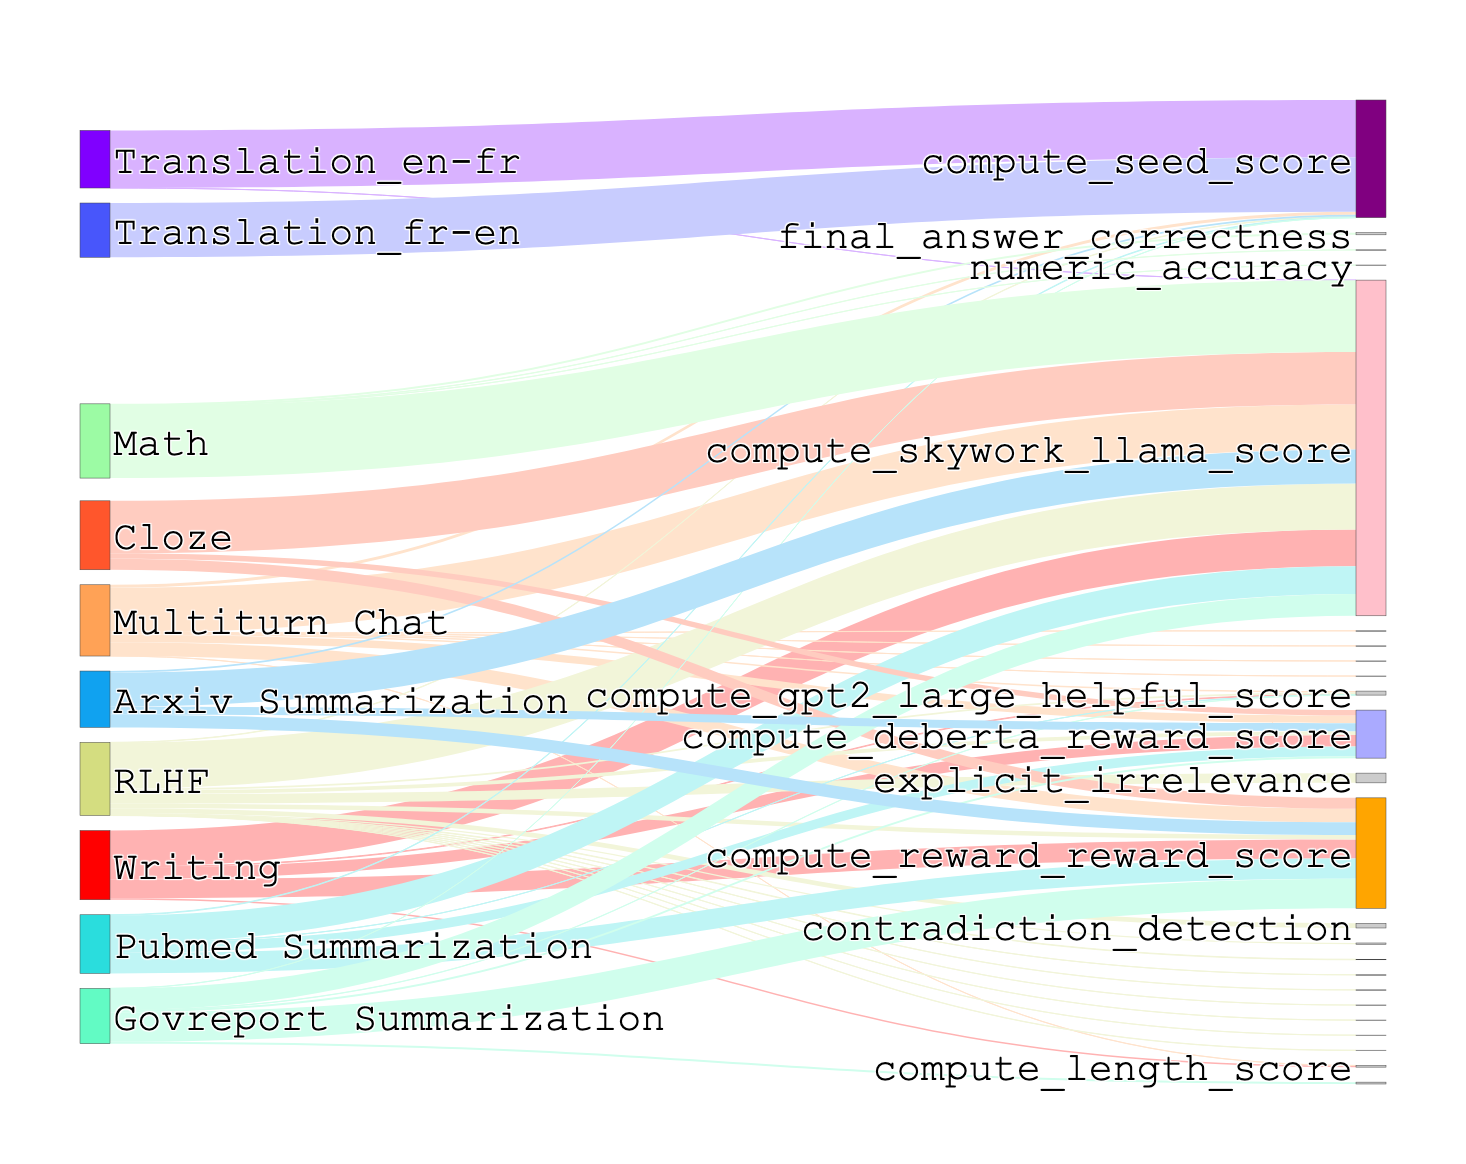
\includegraphics[width=0.45\textwidth]{Figures/sanky.png}
   \caption{Matching tools with source training dataset distribution.}
  \label{fig:sanky}
\end{figure}


The dominance of LLM-based rewards suggests that, for heterogeneous open-domain training, high-capacity discriminative models remain the most trusted. 
Nevertheless, the occasional use of rule-based checks in math and RLHF tasks demonstrates that \method{} is capable of \emph{combining expert heuristics} when appropriate.
\method{} does not rely on a single global reward model but instead orchestrates a \emph{portfolio} of evaluators aligned with each domain.
As shown in the previous subsection, this diversity translates into smoother advantage estimation and stronger updates during policy optimization.



\subsection{Impact on Advantage Estimation and Policy Learning}
% \subsection{Advantage Estimation: Generalists or Experts?


\begin{figure}[t]
    \centering
    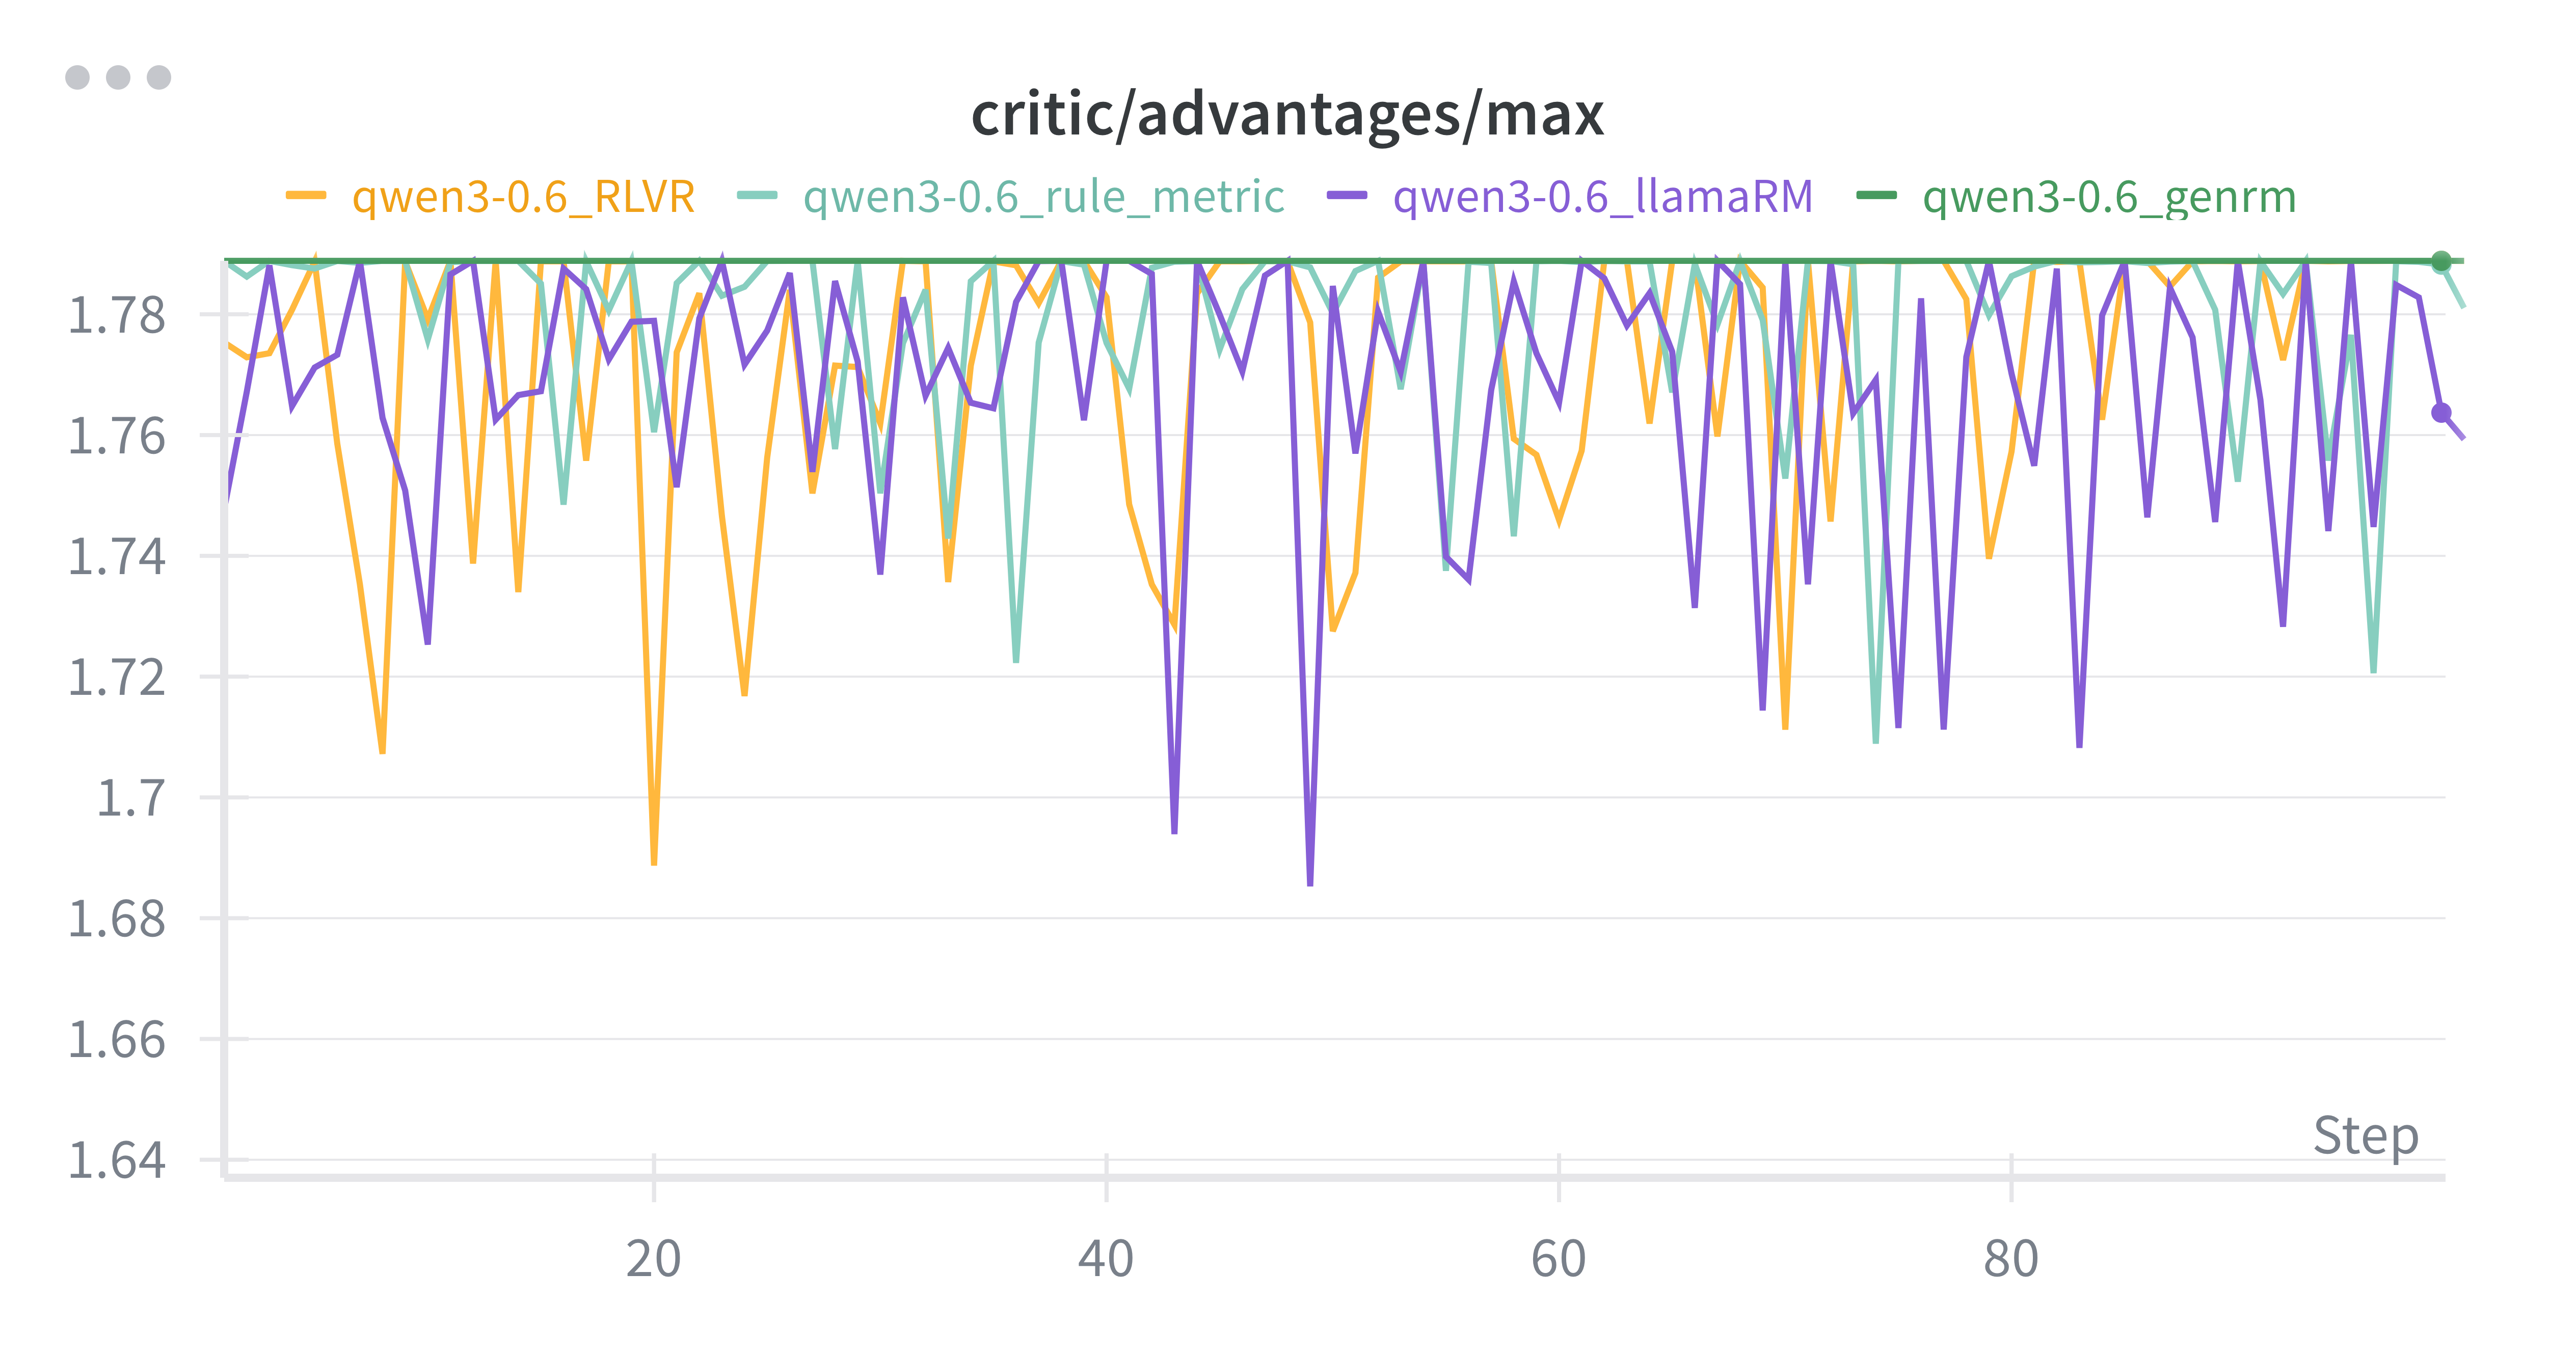
\includegraphics[width=1.0\linewidth]{Figures/adv_max_qwen.png}
    \caption{Maximum Advantage Estimations}
    \label{fig:max_adv}
\end{figure}

\begin{figure}[t]
    \centering
    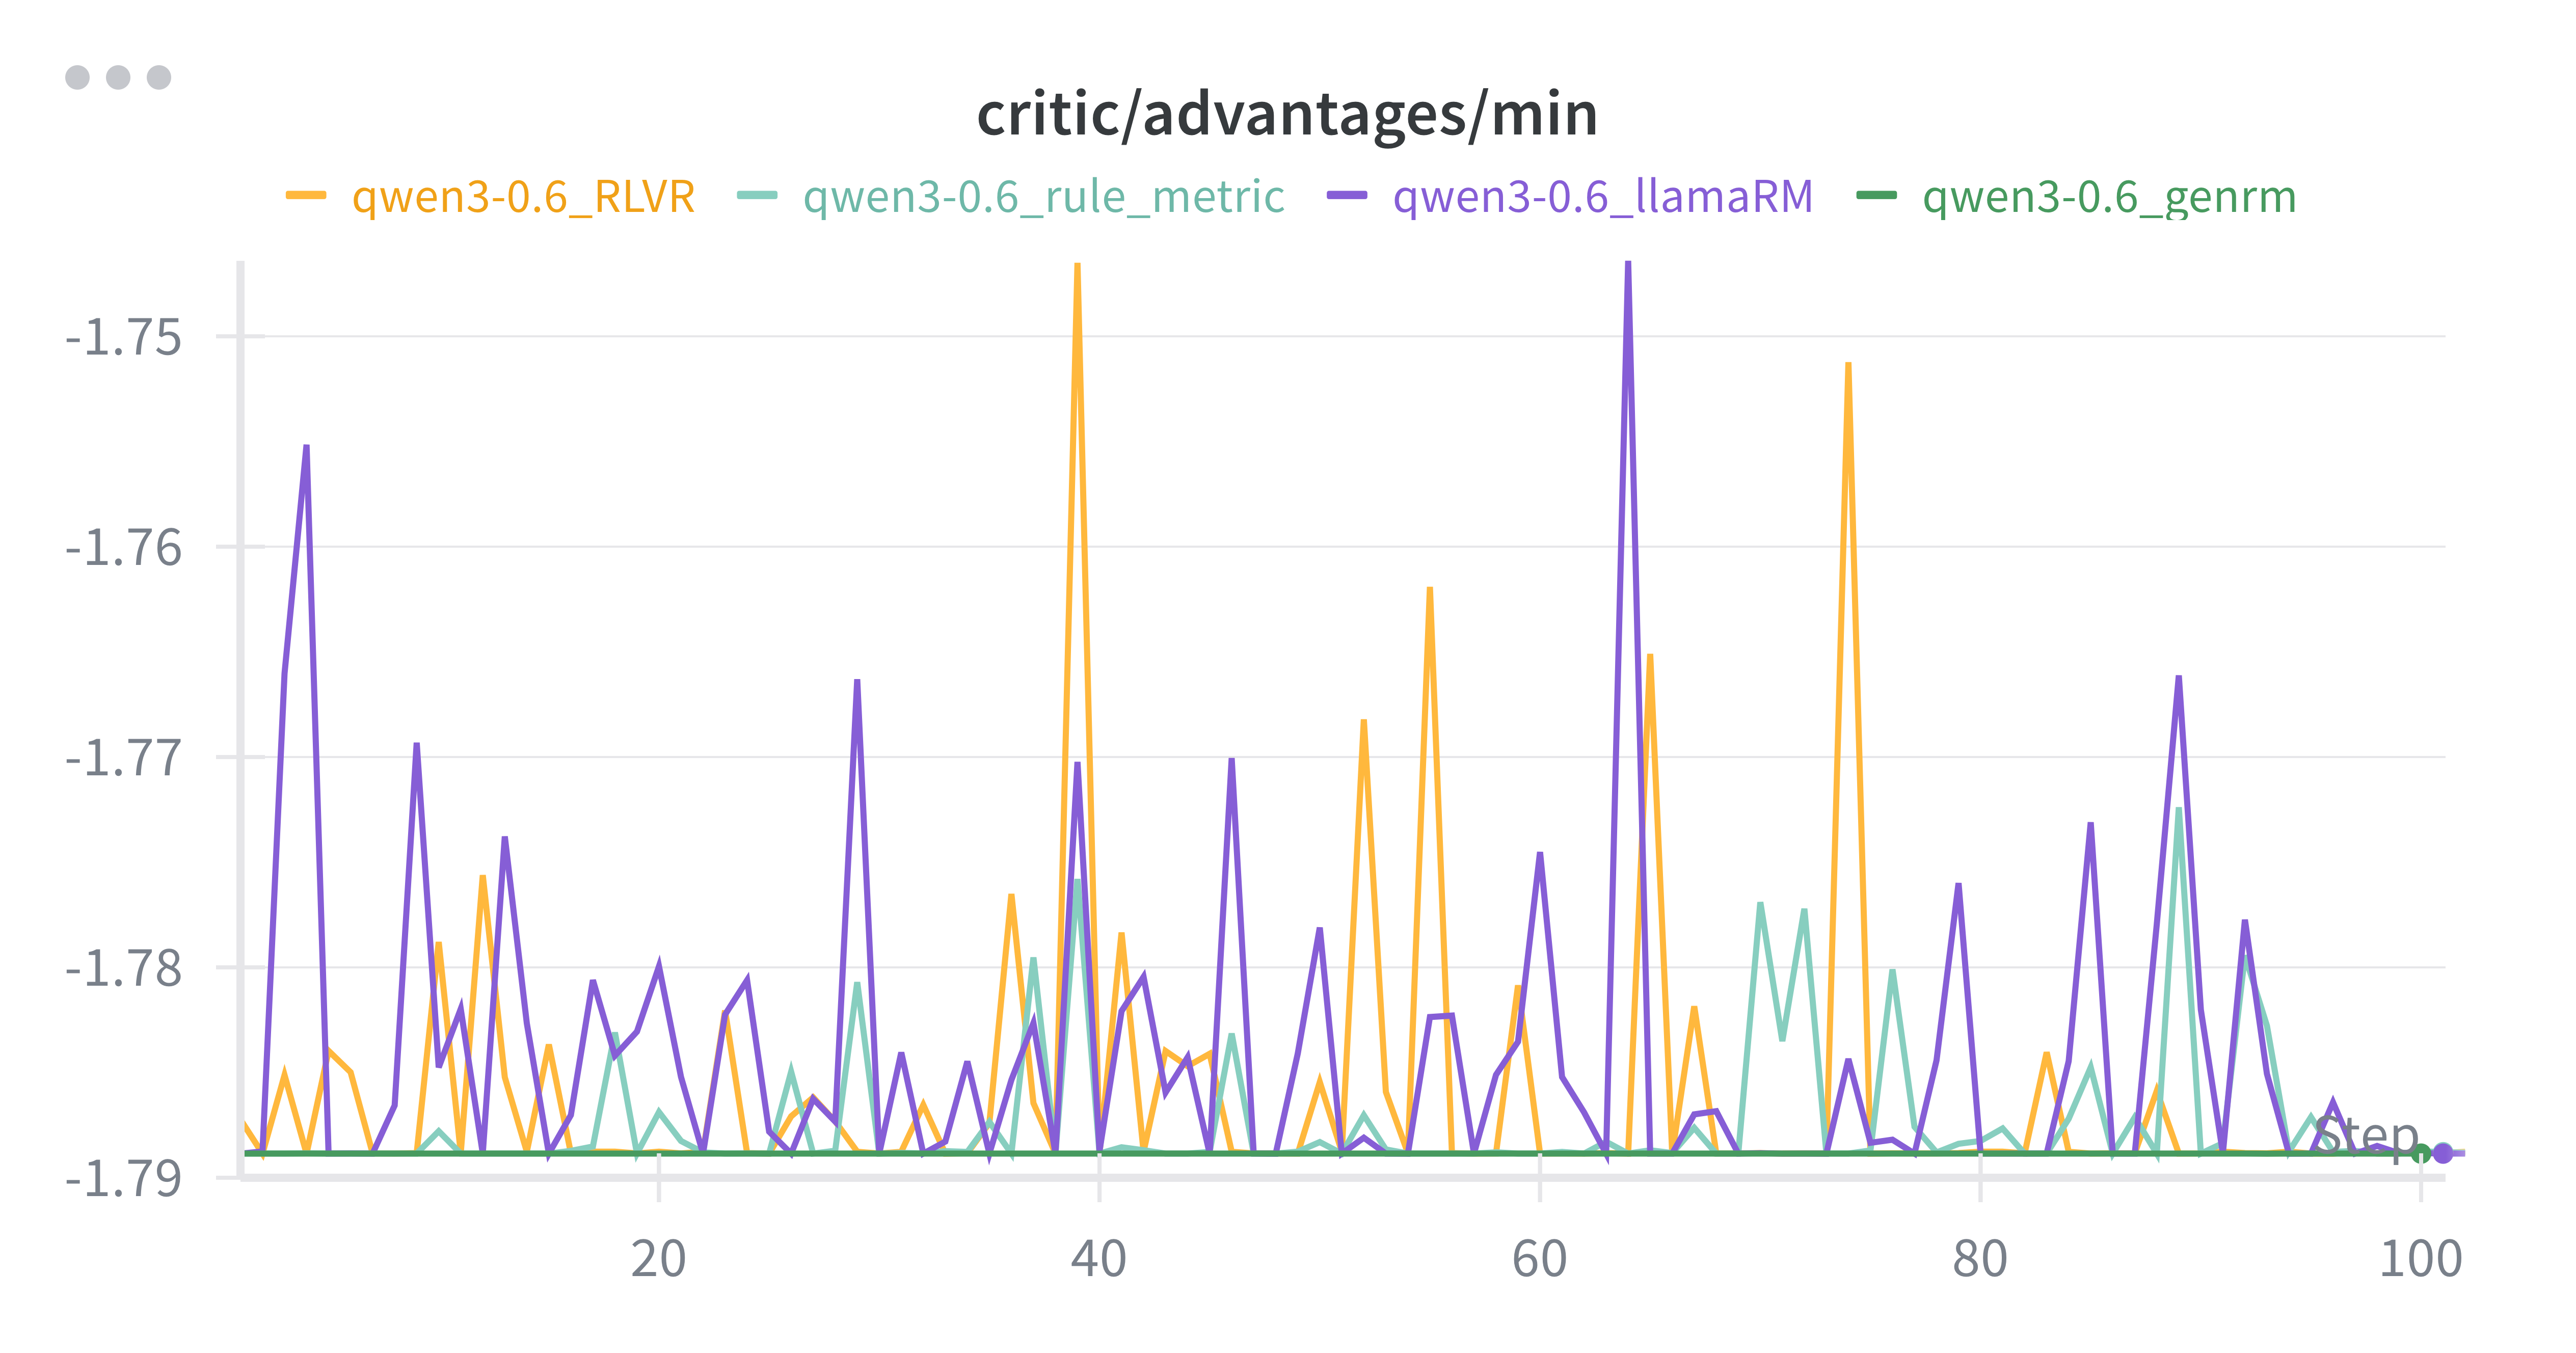
\includegraphics[width=1.0\linewidth]{Figures/adv_min_qwen.png}
    \caption{Minimum Advantage Estimations}
    \label{fig:min_adv}
\end{figure}


We examine the records from the Qwen experiments covering Generative RM, \method{}, and single generic reward, regarding the estimated min/max of advantage per step (Figure~\ref{fig:max_adv} and Figure~\ref{fig:min_adv}), and calculate the proportion that triggered clipping. Higher rates of being clipped mean a higher absolute value of estimated advantage. From the results, for Generative RM, rollouts triggering both upper-clip and under-clip occur in every update step. Compared to single generic reward, \method{} has a significantly higher clipping rate. This is direct evidence that \textbf{methods with better performance tend to estimate larger advantages in absolute values}.



\begin{figure}[t]
  \centering
  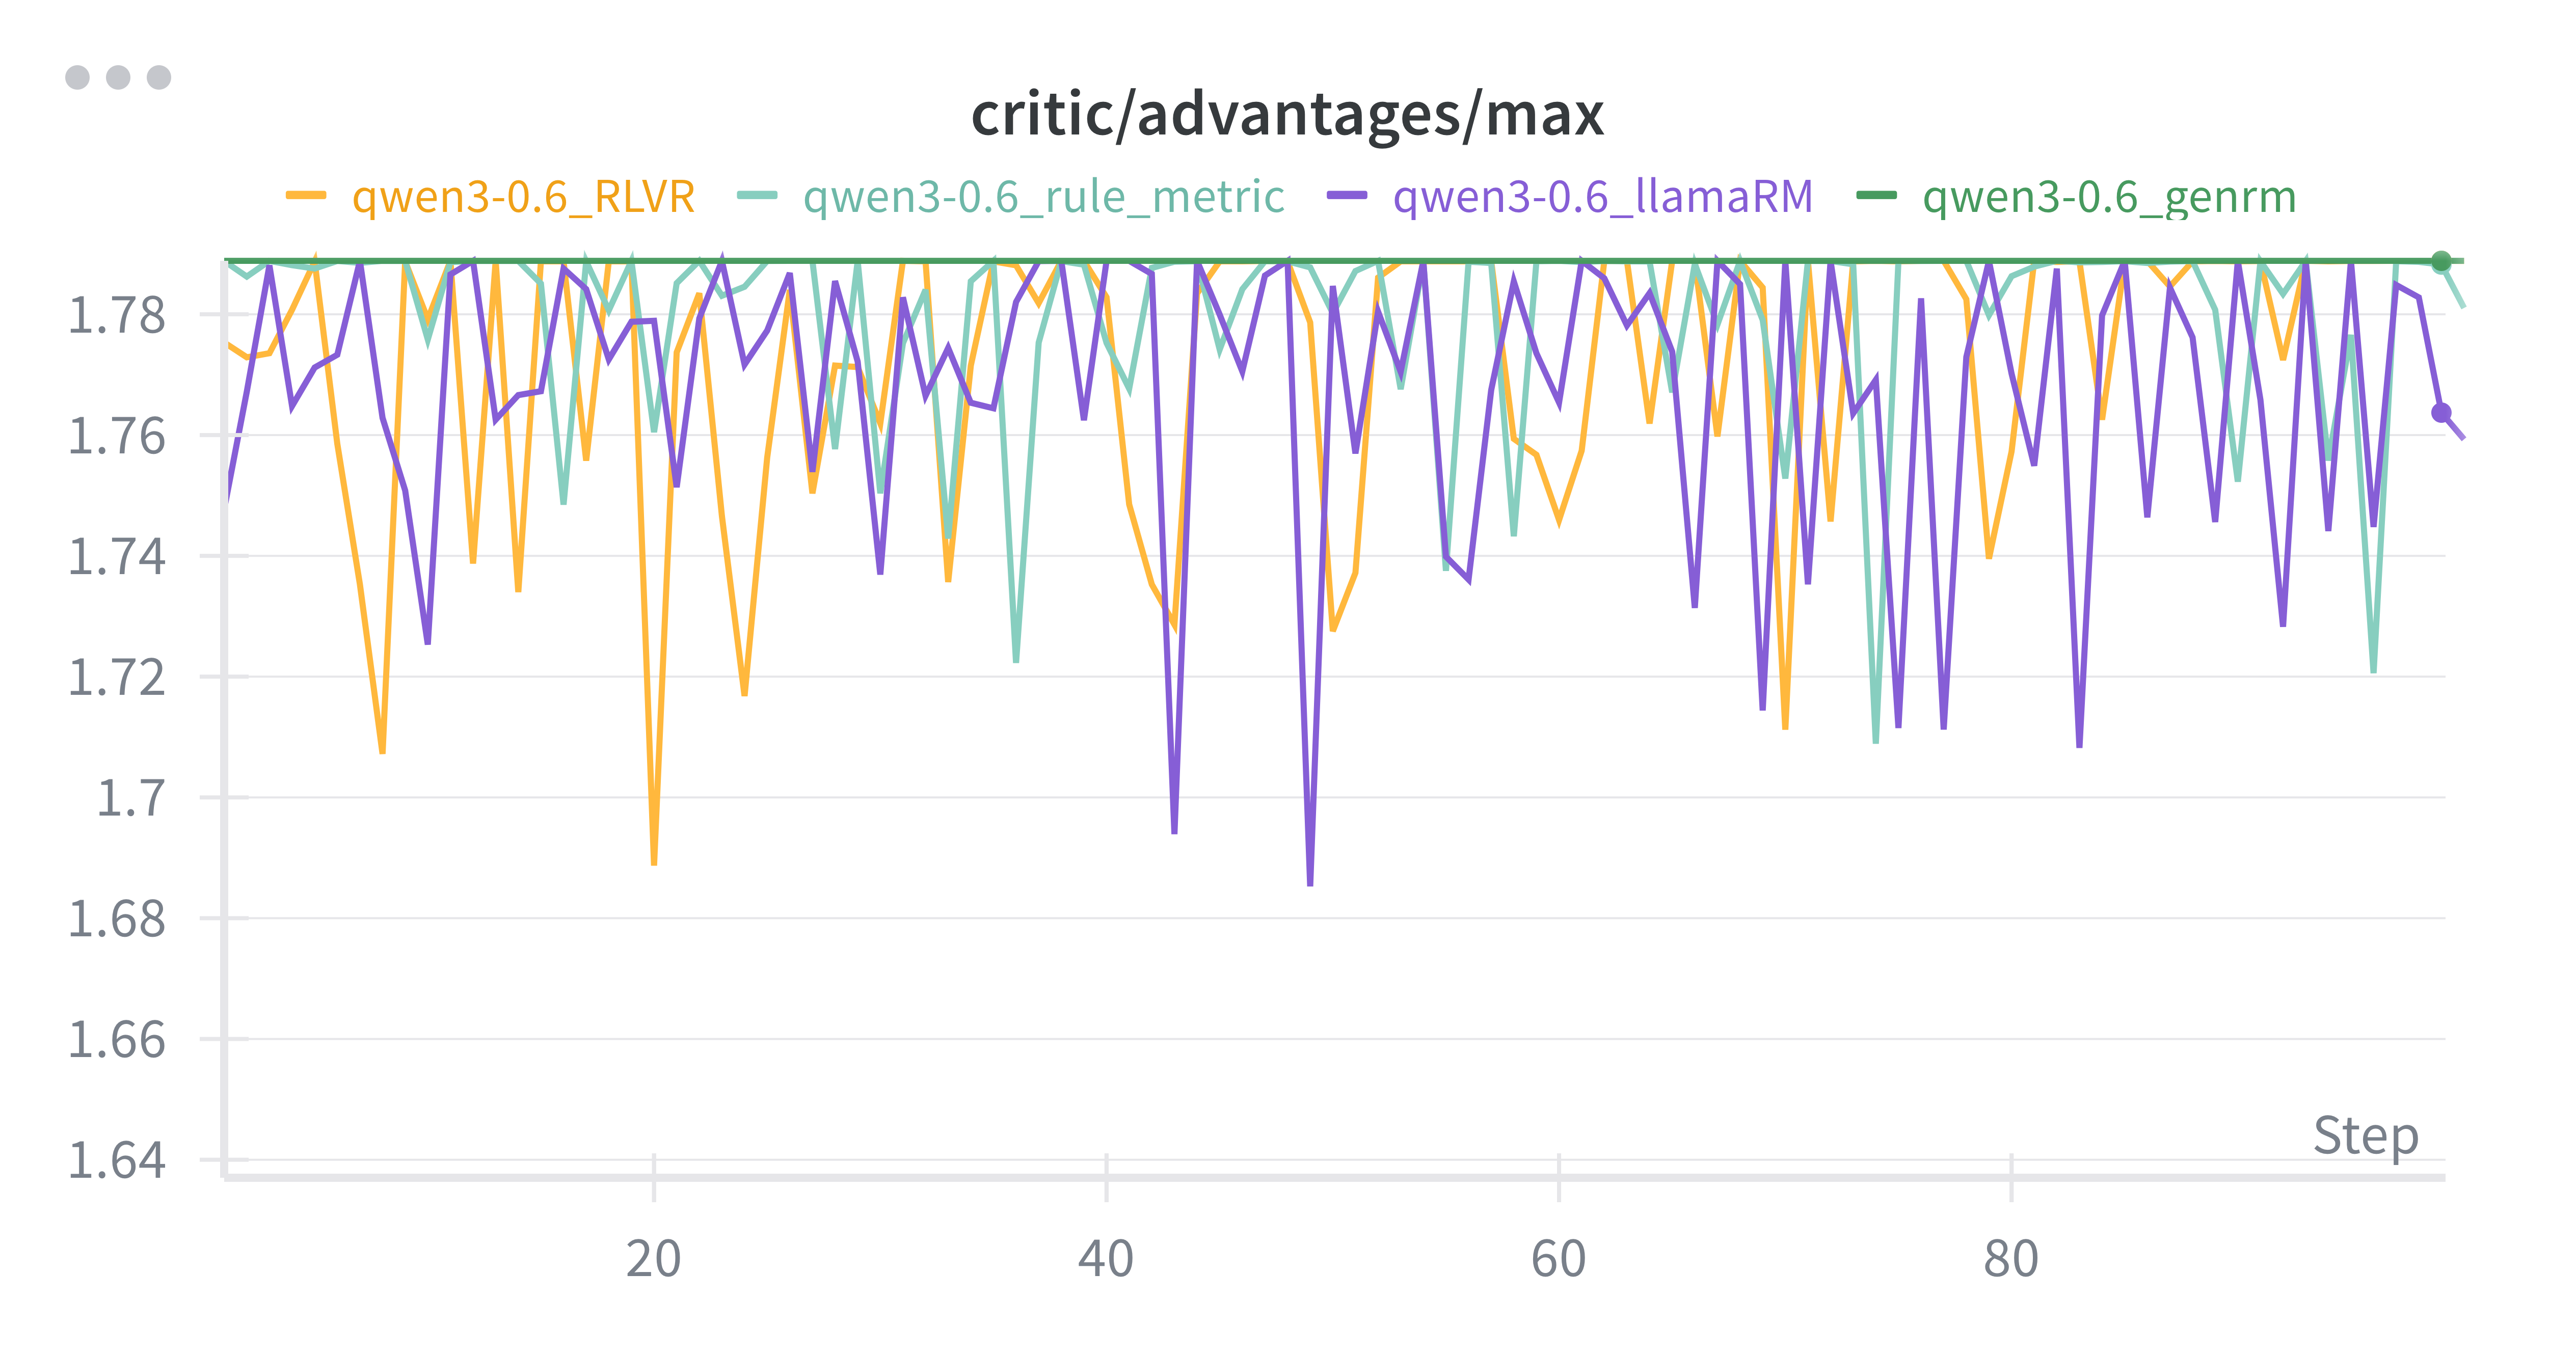
\includegraphics[width=1.0\linewidth]{Figures/adv_max_qwen.png}
   \caption{\small An illustration on the sensitivity to extreme values of reward functions.}
  \label{fig:illustrate}
\end{figure}


Returning to the discussion of Advantage Estimation \(\hat{A}_{i} = \frac{r_i - \mathrm{mean}(r)}{\mathrm{std}(r)}\). Consider two types of reward functions in Figure~\ref{fig:illustrate}: the blue one is sensitive to extreme values (smaller variance) while the orange one is evenly modeled (higher variance).
Assuming uniform roll-out sampling, a higher value of \(\hat{A}_i\) suggests that the underlying reward function resembles \textbf{the sensitive type} (blue line). Therefore, extreme values (maximum/minimum) are divided by a smaller variance, resulting in more frequent reaching of the clip threshold. This is expected for policy optimization, where more weight should be assigned to these deviated rollouts as part of the exploration-exploitation balance.



